\section{Referencia de la Clase bulmafact}
\label{classbulmafact}\index{bulmafact@{bulmafact}}
Clase bulmafact.  


{\tt \#include $<$bulmafact.h$>$}

Diagrama de colaboraci\'{o}n para bulmafact:\begin{figure}[H]
\begin{center}
\leavevmode
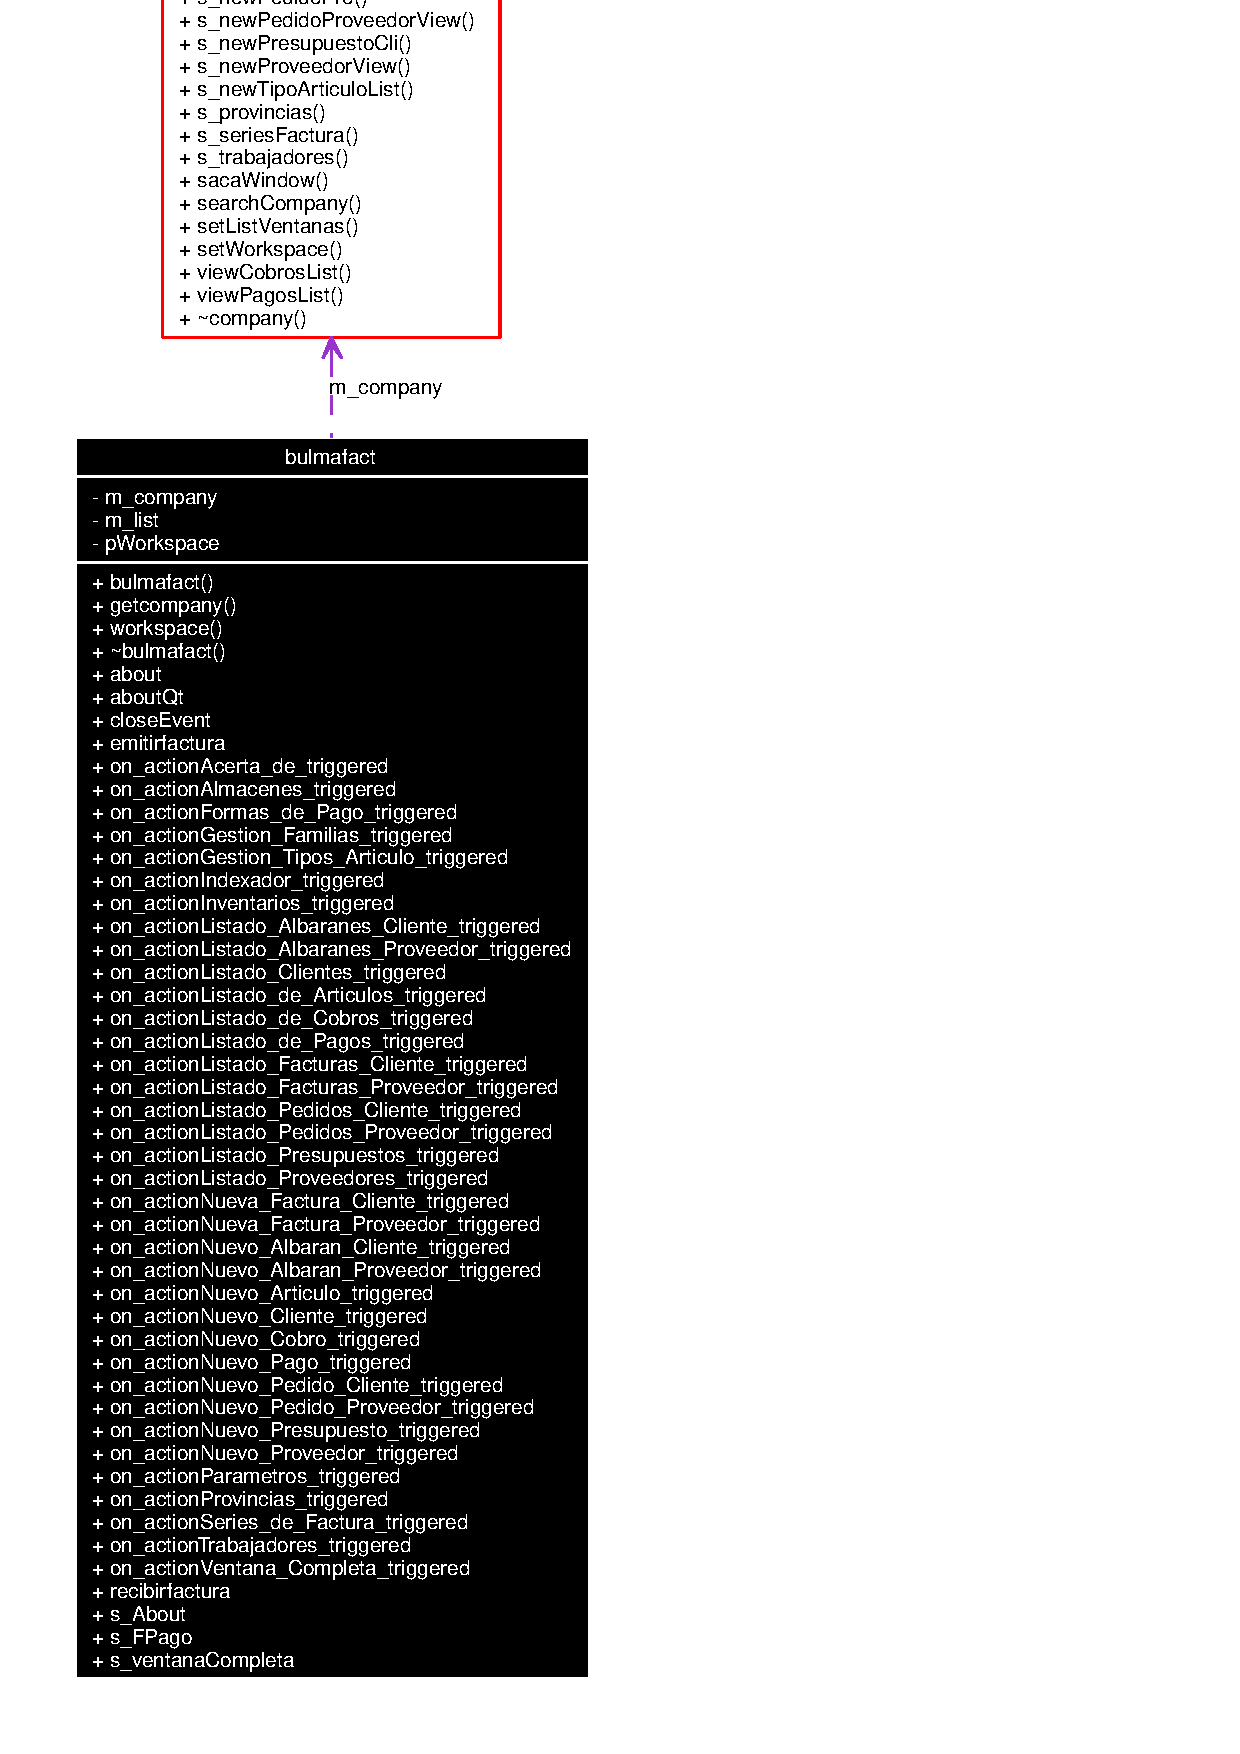
\includegraphics[width=141pt]{classbulmafact__coll__graph}
\end{center}
\end{figure}
\subsection*{Slots p\'{u}blicos}
\begin{CompactItemize}
\item 
void {\bf about} ()\label{classbulmafact_i0}

\item 
void {\bf about\-Qt} ()\label{classbulmafact_i1}

\item 
virtual void {\bf close\-Event} (QClose\-Event $\ast$)\label{classbulmafact_i2}

\item 
virtual void {\bf emitirfactura} ()\label{classbulmafact_i3}

\item 
virtual void {\bf on\_\-action\-Acerta\_\-de\_\-triggered} ()\label{classbulmafact_i4}

\item 
virtual void {\bf on\_\-action\-Almacenes\_\-triggered} ()\label{classbulmafact_i5}

\item 
virtual void {\bf on\_\-action\-Formas\_\-de\_\-Pago\_\-triggered} ()\label{classbulmafact_i6}

\item 
virtual void {\bf on\_\-action\-Gestion\_\-Familias\_\-triggered} ()\label{classbulmafact_i7}

\item 
virtual void {\bf on\_\-action\-Gestion\_\-Tipos\_\-Articulo\_\-triggered} ()\label{classbulmafact_i8}

\item 
virtual void {\bf on\_\-action\-Indexador\_\-triggered} ()\label{classbulmafact_i9}

\item 
virtual void {\bf on\_\-action\-Inventarios\_\-triggered} ()\label{classbulmafact_i10}

\item 
virtual void {\bf on\_\-action\-Listado\_\-Albaranes\_\-Cliente\_\-triggered} ()\label{classbulmafact_i11}

\item 
virtual void {\bf on\_\-action\-Listado\_\-Albaranes\_\-Proveedor\_\-triggered} ()\label{classbulmafact_i12}

\item 
virtual void {\bf on\_\-action\-Listado\_\-Clientes\_\-triggered} ()\label{classbulmafact_i13}

\item 
virtual void {\bf on\_\-action\-Listado\_\-de\_\-Articulos\_\-triggered} ()\label{classbulmafact_i14}

\item 
virtual void {\bf on\_\-action\-Listado\_\-de\_\-Cobros\_\-triggered} ()\label{classbulmafact_i15}

\item 
virtual void {\bf on\_\-action\-Listado\_\-de\_\-Pagos\_\-triggered} ()\label{classbulmafact_i16}

\item 
virtual void {\bf on\_\-action\-Listado\_\-Facturas\_\-Cliente\_\-triggered} ()\label{classbulmafact_i17}

\item 
virtual void {\bf on\_\-action\-Listado\_\-Facturas\_\-Proveedor\_\-triggered} ()\label{classbulmafact_i18}

\item 
virtual void {\bf on\_\-action\-Listado\_\-Pedidos\_\-Cliente\_\-triggered} ()\label{classbulmafact_i19}

\item 
virtual void {\bf on\_\-action\-Listado\_\-Pedidos\_\-Proveedor\_\-triggered} ()\label{classbulmafact_i20}

\item 
virtual void {\bf on\_\-action\-Listado\_\-Presupuestos\_\-triggered} ()\label{classbulmafact_i21}

\item 
virtual void {\bf on\_\-action\-Listado\_\-Proveedores\_\-triggered} ()\label{classbulmafact_i22}

\item 
virtual void {\bf on\_\-action\-Nueva\_\-Factura\_\-Cliente\_\-triggered} ()\label{classbulmafact_i23}

\item 
virtual void {\bf on\_\-action\-Nueva\_\-Factura\_\-Proveedor\_\-triggered} ()\label{classbulmafact_i24}

\item 
virtual void {\bf on\_\-action\-Nuevo\_\-Albaran\_\-Cliente\_\-triggered} ()\label{classbulmafact_i25}

\item 
virtual void {\bf on\_\-action\-Nuevo\_\-Albaran\_\-Proveedor\_\-triggered} ()\label{classbulmafact_i26}

\item 
virtual void {\bf on\_\-action\-Nuevo\_\-Articulo\_\-triggered} ()\label{classbulmafact_i27}

\item 
virtual void {\bf on\_\-action\-Nuevo\_\-Cliente\_\-triggered} ()\label{classbulmafact_i28}

\item 
virtual void {\bf on\_\-action\-Nuevo\_\-Cobro\_\-triggered} ()\label{classbulmafact_i29}

\item 
virtual void {\bf on\_\-action\-Nuevo\_\-Pago\_\-triggered} ()\label{classbulmafact_i30}

\item 
virtual void {\bf on\_\-action\-Nuevo\_\-Pedido\_\-Cliente\_\-triggered} ()\label{classbulmafact_i31}

\item 
virtual void {\bf on\_\-action\-Nuevo\_\-Pedido\_\-Proveedor\_\-triggered} ()\label{classbulmafact_i32}

\item 
virtual void {\bf on\_\-action\-Nuevo\_\-Presupuesto\_\-triggered} ()\label{classbulmafact_i33}

\item 
virtual void {\bf on\_\-action\-Nuevo\_\-Proveedor\_\-triggered} ()\label{classbulmafact_i34}

\item 
virtual void {\bf on\_\-action\-Parametros\_\-triggered} ()\label{classbulmafact_i35}

\item 
virtual void {\bf on\_\-action\-Provincias\_\-triggered} ()\label{classbulmafact_i36}

\item 
virtual void {\bf on\_\-action\-Series\_\-de\_\-Factura\_\-triggered} ()\label{classbulmafact_i37}

\item 
virtual void {\bf on\_\-action\-Trabajadores\_\-triggered} ()\label{classbulmafact_i38}

\item 
virtual void {\bf on\_\-action\-Ventana\_\-Completa\_\-triggered} ()\label{classbulmafact_i39}

\item 
virtual void {\bf recibirfactura} ()\label{classbulmafact_i40}

\item 
virtual void {\bf s\_\-About} ()\label{classbulmafact_i41}

\item 
virtual void {\bf s\_\-FPago} ()\label{classbulmafact_i42}

\item 
virtual void {\bf s\_\-ventana\-Completa} ()\label{classbulmafact_i43}

\end{CompactItemize}
\subsection*{M\'{e}todos p\'{u}blicos}
\begin{CompactItemize}
\item 
{\bf bulmafact} (QString bd)
\item 
{\bf company} $\ast$ {\bf getcompany} ()\label{classbulmafact_a1}

\item 
QWorkspace2 $\ast$ {\bf workspace} ()\label{classbulmafact_a2}

\item 
{\bf $\sim$bulmafact} ()
\end{CompactItemize}


\subsection{Descripci\'{o}n detallada}
Clase bulmafact. 



\subsection{Documentaci\'{o}n del constructor y destructor}
\index{bulmafact@{bulmafact}!bulmafact@{bulmafact}}
\index{bulmafact@{bulmafact}!bulmafact@{bulmafact}}
\subsubsection{\setlength{\rightskip}{0pt plus 5cm}bulmafact::bulmafact (QString {\em bd})}\label{classbulmafact_a0}


Aqui creamos la ventana dock para meter las distintas ventanas.

Iniciamos el listventanas con el workspace para que pueda operar con el \index{bulmafact@{bulmafact}!~bulmafact@{$\sim$bulmafact}}
\index{~bulmafact@{$\sim$bulmafact}!bulmafact@{bulmafact}}
\subsubsection{\setlength{\rightskip}{0pt plus 5cm}bulmafact::$\sim$bulmafact ()}\label{classbulmafact_a3}


En MS-Windows no termina bien la ejecucion del programa y por eso agregamos esta salida rapida. 

La documentaci\'{o}n para esta clase fu\'{e} generada a partir de los siguientes archivos:\begin{CompactItemize}
\item 
bulmafact.h\item 
bulmafact.cpp\end{CompactItemize}
